\chapter{Contexte général}
\section*{Introduction}
Ce premier chapitre permettra de définir le contexte général de notre travail. Nous fournirons une brève présentation de la Société le Monde Informatique (SMI). Ensuite, nous décrirons brièvement le travail demandé ainsi que ses principales fonctionnalités, avant de finir par une présentation de la méthodologie de développement adoptée.

% Une section

% Exemple d'une section qui porte une référence à une bibliographie
% NB: il faut bien suivre le syntaxe pour ne pas tomber dans le cas où il y a une référence dans la table des matières.
\section{Cadre du projet}
Dans le cadre de notre formation en Génie Logiciel et Systèmes d’Information (GLSI) à l'Institut Supérieur de l'Informatique (ISI), nous avons eu l'occasion d'effectuer notre stage de fin d'études au sein de la SMI, en vue de l'obtention du Diplôme National d’Ingénieur en Sciences Appliquées et Technologiques. En effet, ce stage vise à compléter notre formation acquise au sein de l'ISI, et de nous introduire à la vie professionnelle par la mise en pratique de nos connaissances dans le cadre d’un travail en équipe. Ce stage consiste en la réalisation d’une application Web pour la conception et le partage de tableaux de bord.
\section[Organisme d'accueil]{Présentation de l'organisme d'accueil}
\subsection{Présentation de la SMI}
% NB: il faut annoncer la figure dabord.
% Pour faire appel à une figure, il suffit d'utiliser le label comme suit :
La figure \ref{fig:logo_tt} présente le logo de la Société le Monde Informatique.\\
% On peut ajouter une figure en utilisant le syntaxe suivant:
\begin{figure}[htpb]
\centering
\frame{
\includegraphics{smi}}
\caption{Logo de la SMI}
\label{fig:logo_tt}
\end{figure}
\newline
La Société le Monde Informatique (SMI) a été créer le 17 Décembre 1991, elle se positionne comme étant un éditeur de logiciel, offrant un portefeuille riche de produits financiers, afin de répondre aux besoins du marché bancaire.\\
Les objectifs de la SMI consistent à offrir des services de gestion et de sécurité visant à augmenter la productivité et la rentabilité des organismes financiers-clients et à apporter des solutions innovantes et performantes.



\subsection{Organisation}
Le bureau de la SMI se situe au centre-ville de Tunis, proche des sièges sociaux des banques représentant des clients potentiels. La société compte aujourd'hui une dizaine d'employés: direction, ingénieurs et techniciens qui réalisent des projets dans le domaine du bancaire étranger notament le projet IBANSYS.\newline
Les projets de la SMI ont été élaborés à la demande de plusieurs clients importants tels que : Promo Sport, AMEN BANK, BIAT, STB, Assurance COMAR, etc.

\subsection{Services}
SMI propose un large éventail de services de solutions :
\begin{itemize}
    \item administrer et migrer les bases de données Oracle,
    \item développer et maintenir des applications qui ont pour fonction d'apporter des solutions innovantes aux clients de l'entreprise dans le contexte de la dématérialisation des documents,
    \item piloter les projets et étudier les plans informatiques.
\end{itemize}

\section{Présentation du sujet}
Notre application s’inscrit dans le cadre de la gestion et le suivi des activités d’une banque ou de tout autre organisme financier.
\subsection{Etude de l’existant}
L’analyse de l’existant est une étape primordiale du projet. Elle permet de lui définir un cadre de conduite, de le mettre en route, afin d’éviter tout type de redondance ou d’imprécisions au niveau de la définition des besoins.\\
Actuellement les statistiques dans une banque réalisées à l’aide de tableaux Excel et sont partagées entre les différentes structures d’une banque (service, département, division …), et chaque structure fille envoie les statistiques relatives à son activité à sa structure mère.\\
Une fois que toutes les statistiques des structures filles soient reçues, la structure mère les consolide en générant un tableau de bord complet.
\subsection{Critique de l’existant}
Le processus de génération de statistiques au sein des différents structures est susceptible d’être itéré à maintes reprises, et il semble non convenable que ce traitement se produise manuellement (perte de temps, perte de ressources et perte probable des documents).
\subsection{Solution proposée}
Pour pallier les problèmes élucidés, nous proposons une solution qui réside dans le développement d’une application web qui fournira aux utilisateurs d’une banque la possibilité de création de statistiques relatifs à l’activité de leurs structures à travers un outil Web interactif et permettra également la création et le partage d’un Dashbord accessible à d’autres utilisateurs.

\section{Étude méthodologique}
Les méthodologies de gestion de projet, jouent un rôle primordial dans la réussite ou l’échec d’un projet. Après avoir identifié les besoins à satisfaire par notre projet, il est donc très important de bien choisir la méthodologie de gestion de notre projet.

\subsection{Méthodologies classiques}
Les méthodologies classiques se divisent en plusieurs phases identifiées dès le démarrage du projet (Définition des besoins, conception générale puis détaillée, réalisation /développement, tests et mise en production). La validation d’une phase entraîne le début de la suivante. Cette méthode limite les retours aux étapes précédentes. La figure \ref{fig:mc} \cite{Mclassiques} présente le principe de fonctionnement des méthodes classiques.
\begin{figure}[htpb]
\centering
    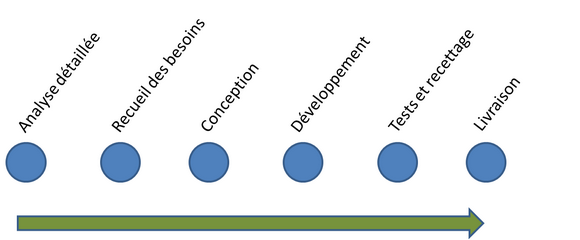
\includegraphics{methode-classique}
    \caption{Principe de fonctionnement des méthodes classiques}
    \label{fig:mc}
\end{figure}
\newpage
\subsection{Méthodologies agiles}
Les méthodes agiles reposent sur un cycle de développement itératif, incrémental et adaptatif. Elles doivent respecter quatre valeurs fondamentales déclinées en douze principes desquels découlent une base de pratiques, soit communes, soit complémentaires. La figure \ref{fig:ma} \cite{Magiles} présente le principe de fonctionnement des méthodes agiles.
\begin{figure}[htpb]
\centering
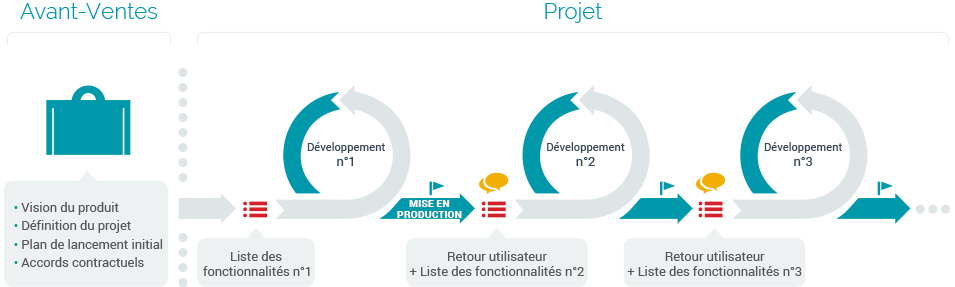
\includegraphics[scale=0.5]{Agile_Diagram}
\caption{Principe de fonctionnement des méthodes agiles} 
\label{fig:ma}
\end{figure}
\subsection{Etude comparative}
Le tableau \ref{table:avsc} \cite{Comparaisonac} présente une comparaison entre les approches classiques et les approches agiles.
    \begin{longtable}{| m{3cm} | m{6cm}| m{6cm} | } 
    \caption{Comparaison entre les approches de développement} 
     \hline
     Thème & Approche classique & Approche agile \\
     \hline
     Cycle de vie & En cascade ou en V, sans rétroaction possible, phase séquentielle. & Itératif et incrémental.\\
     \hline
     Planification &	Prédictive, caractérisée par des plans plus ou moins détaillées sur la base d'un périmètre et d'exigences définies et stables au début du projet. &	Adaptative avec plusieurs niveaux de planification avec ajustement si nécessaire en fonction des changements survenues.\\
     \hline
     Documentation &	Produite en quantité importante comme support de communication, de validation et de contractualisation &	Réduite au strict nécessaire au profit d’incréments fonctionnes opérationnels pour obtenir le feedback du client\\
     \hline
Equipe &	Une équipe avec des ressources spécialisées, dirigées par un chef de projet	& Une équipe responsabilisée ou l’initiative et la communication sont privilégiées, soutenue par le chef de projet \\ 
\hline
Qualité &	Contrôle de qualité à la fin du cycle de développement. Le client découvre le produit fini.	& Un contrôle qualité précoce et permanent, au niveau du produit et du processus. Le client visualise les résultats tôt et fréquemment. \\
\hline
Changement &	Résistant voire opposition au changement.
Processus lourds de gestion des changement acceptés. &	Accueil favorable au changement inéluctable, intégré dans un processus.\\
\hline 
Suivi de l’avancement	& Mesure de la conformité aux plans initiaux.
Analyse des écarts. &	Un seul indicateur de l’avancement : le nombre de fonctionnalités implémentées et le travail restant à faire.\\
\hline
Gestion des risques	& Processus distinct, rigoureux de gestion des risques.	& Gestion des risques intégrée dans le processus global, avec responsabilisation de chacun dans l’identification et la résolution des risques.
Pilotage par les risques.\\
\hline
Mesure de succès &	Respect des engagement initiaux en termes de coûts, de budget et de niveau de qualité. &	Satisfaction client par la livraison de valeur ajoutée.\\
\hline
    \end{longtable}
    
    \label{table:avsc}

Les méthodologies classiques possèdent des avantages dont leur bonne base d’organisation du projet et leur sens rationnel, mais elles exigent un ensemble de facteurs clés de succès difficiles à faire réunir avant le démarrage d’un projet, comme par exemple :
\begin{itemize}
    \item les bonnes idées doivent être identifiées préalablement au démarrage de tout projet,
    \item l'entreprise doit être capable de prévoir le futur avec précision, y compris les imprévus métiers comme technologiques,
    \item les responsables de projet doivent planifier les tâches incertaines avec exactitude,
\end{itemize}
Conscients des inconvénients des méthodologies classiques déjà cités, nous avons choisi d’adopter le concept Agile Scrum dans la conduite et la gestion de notre projet.
\subsection{Choix méthodologique: Scrum}
La première priorité d’agile est de satisfaire le client en livrant tôt et régulièrement des logiciels utiles. De plus, avec Agile, le changement est accepté, même tardivement dans le développement. Les processus agiles exploitent le changement comme avantage compétitif pour le client et promeuvent un rythme de développement soutenable.  Ils donnent aussi une attention continue à l'excellence technique et à la qualité de la conception.\\
Nous avons choisi comme méthodologie de développement la méthodologie Scrum, la figure \ref{fig:su} \cite{scrumvsall} suivante présente une comparaison entre le pourcentage d'utilisation des différents méthodes agiles.

\begin{figure}[htpb]
\centering
\frame{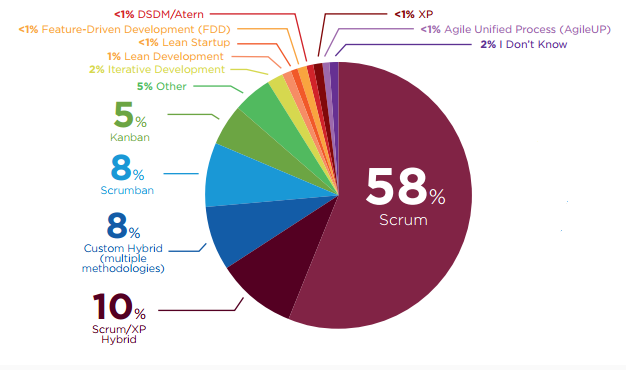
\includegraphics{scrumvsall}}
\caption{Le pourcentage d'utilisation des méthodes agiles}
\label{fig:su}
\end{figure}
\newpage
Les raisons de ce choix sont principalement :
\begin{itemize}
    \item le besoin de communication : L’équipe doit s’organiser pour atteindre ses objectifs, en favorisant une collaboration maximale entre ses membres ainsi que ses clients,
    \item la nécessité des feedbacks : tout peut être remis en jeu à tout moment puisque les fonctionnalités du projet peuvent toujours s’évoluer,
    \item des plannings souples modifiables au fur et à mesure des évènements : puisque seuls les grands objectifs sont fixés au début de notre stage, il est préférable d’avoir un plan souple et évolutif pour faciliter le développement pas à pas,
\end{itemize}

La méthodologie Scrum est la méthodologie agile la plus populaire. Scrum est basée sur des réunions quotidiennes ce qui favorise le travail collaboratif et la communication entre les membres de l’équipe afin d’améliorer la productivité. \\
Scrum met en place un mécanisme de contrôle continu sur l’avancement de travail ainsi que sur la qualité du produit ce qui facilite, dans notre cas, à l’encadrant académique et les encadrants professionnels de bien suivre le déroulement du projet. \\
Le principe de fonctionnement de Scrum s’appuie sur le découpage des projets en itérations nommées « sprints » d’une période allant de deux à quatre semaines. Chaque sprint possède un but à atteindre, défini par le directeur du produit (le Product Owner), à partir duquel sont choisies les fonctionnalités à implémenter dans ce sprint. La figure suivante nous montre le principe de fonctionnement de la méthodologie Scrum.
\begin{figure}[htpb]
\centering
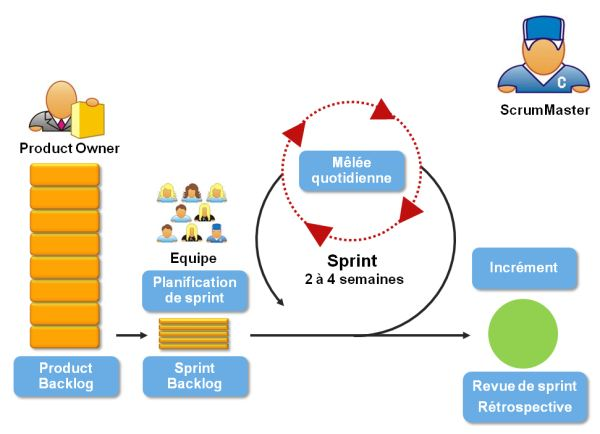
\includegraphics[scale=.7]{methode-scrum}
\caption{Principe de fonctionnement de la méthodologie Scrum.}
\label{fig:mc}
\end{figure}
\subsection{Application de Scrum}
Le cadre Scrum est constitué de trois éléments qui sont les rôles, les blocs de temps et les artefacts. Il s’agit dans notre cas, d’appliquer Scrum dans un cadre de projet de fin d’études. Nous avons donc essayé d’adapter ces éléments en fonction de nos besoins.

\subsubsection{L'équipe}

    Scrum définit trois rôles : le propriétaire du produit (product owner), le scrum master et le Scrum team.\newpage
 \begin{longtable}{| m{3cm} | m{9cm}| m{3cm} | } 
    \caption{L'équipe}
    \hline
    Rôle &	Description	& Personne affectée \\
    \hline
Product Owner &	La personne qui communique les objectifs premiers des clients et utilisateurs finaux, coordonne l’implication des utilisateurs et des parties prenantes, et se coordonne lui-même avec les autres product owners pour assurer une cohérence. & Banque	\\
    \hline
Scrum Master &	C’est un membre de l’équipe, il a pour but d’optimiser la capacité de production de l’équipe. Pour se faire, le scrum master aide l’équipe à travailler de façon autonome tout en s’améliorant d’avantage. &
Anis ZEMNI \\
    \hline
Scrum Team	& La particularité d’une équipe scrum est qu’elle est dépourvue de toute hiérarchie interne. Une équipe scrum est auto-organisée. &	Nejm Eddine HIDRI \\
\hline

 \end{longtable}
 
 \subsubsection{Artefacts}
 \begin{itemize}
     \item Le « product backlog » : c’est un document qui contient les exigences initiales dressées puis hiérarchisées avec le client au début du projet. Néanmoins il va évoluer tout au long de la durée du projet, en fonction des divers besoins du client.
\item Le « sprint backlog » : A chaque début de sprint, l’équipe définit un but. Puis lors de la réunion de sprint, l’équipe de développement choisit les éléments du carnet à réaliser. 
\item « User story » : les fonctionnalités décrites par le client.
\item	« Burndown Chart » :c’est un graphique d’avancement, généré dès le début de chaque sprint, permettant de visualiser la progression de l’équipe.Il doit être mis à jour quotidiennement et est un excellent indicateur de rendement et de suivi pour le Product Owner, qui peut réagir si nécessaire, lorsqu’il constate que le sprint possède un nombre important de scénarios ; dans ce cas il diminue les user stories, ou à l’inverse il pourra en rajouter.
 \end{itemize}
 
 \subsubsection{Evènements}
 \begin{itemize}
 \item La mêlée : c’est une réunion d’avancement organisée de manière quotidienne durant le sprint. Durant cette réunion l’équipe examine attentivement, le travail effectué depuis la dernière mêlée, et prévoit le travail qui doit être réalisé pour la prochaine mêlée.
 \item Les revues de Sprint : Cette réunion se tient à la fin de chaque Sprint.L’équipe présente ce qu'elle a fait durant cette période. L’utilité de cette réunion, est de réaliser une démonstration de l’incrément développé. L'équipe présente alors les fonctionnalités développées au Product Owner, qui va donner son avis (refus ou approbation).
 \item Rétrospective de sprint : Cette réunion a lieu à la fin de chaque sprint. A l’inverse de la revue de sprint, ce meeting est organisé et animé par le Scrum Master. Elle a pour but d’améliorer le processus de développement et d’apprentissage de l’équipe en mettant en valeur les idées de chacun sur la table, et en soulevant les points et les différents obstacles rencontrés, en vue de trouver des solutions et d'améliorer le rendement pour les sprints qui suivront.

 \end{itemize}
 
 \subsubsection{Backlog de produit}
Le Backlog de produit est la liste des macro-fonctionnalités (User Story), à exécuter durant le projet, priorisées selon leur valeur métier par rapport à la solution finale.
\paragraph{La méthode MoSCow pour les priorités}
La technique utilisée pour prioriser les besoins dans un contexte itératif est celle de MoSCoW. L'avantage de la méthode MoSCoW réside dans la signification de l'acronyme, qui est plus compréhensible que d'autres techniques de priorisation comme élevé/moyen/faible.
\begin{itemize}
    \item M pour « Must Havee » : doit être faite, l’exigence est essentielle. Si elle n’est pas faîte le projet échoue. On peut dire également priorité haute.
    \item S pour « Should Have » : Il s’agit d’une exigence essentielle, qu’il faut faire dans la mesure du possible. Mais si elle n’est pas faîte, on peut la contourner et la livrer plus tard.
    \item C pour « Could Have » : Il s’agit d’une exigence souhaitable. Elle pourrait être faîte dans la mesure où elle n’a pas d’impact sur les autres tâches.
    \item W pour « Won't Have » Il s’agit d’une exigence « Luxe ». Ne sera pas faîte cette fois mais plus tard, mais intéressante et à garder pour la prochaine version.
\end{itemize}

\paragraph{Construction du Backlog de produit :}

le tableau \ref{tab:productbacklog} présente les fonctionnalités de notre système.

\begin{longtable}{| p{1.5cm}  | p{2cm} | p{1.5cm} | p{6cm} | p{1cm} |  p{1.5cm} |} 
    \caption{Backlog de produit du projet}
    \label{tab:productbacklog}
     \hline
     ID Feature & Feature & ID User Story & User Story  & Effort & Priorité\\ \hline
1 & Gestion des statistiques  & 1.1 & En tant qu'administrateur je peux créer une nouvel statistique & ~ & M \\ \cline{3-6}
& & 1.2 & En tant qu'administrateur je peux créer une nouvel statistique & ~ & M \\ \cline{3-6}
& & 1.3 & En tant qu'administrateur je peux consulter une statistique & ~ & M \\ \cline{3-6}
& &  1.4 & En tant qu'administrateur je peux exécuter une statistique & ~ & M \\ \cline{3-6}
& &  1.5 & En tant qu'administrateur je peux modifier une statistique & ~ & M \\ \cline{3-6}
& &  1.6 & En tant qu'administrateur je peux partager une statistique & ~ & M \\ \cline{3-6}
& &  1.7 & En tant qu'administrateur je peux supprimer une statistique & ~ & M \\ \cline{3-6}
& &  1.8 & En tant qu'administrateur je peux chercher une statistique & ~ & M \\ \hline

2 & Gestion des Dashboards & 2.1 & En tant qu'agent je peux créer un nouveau Dashboard & & M \\ \cline{3-6}
& & 2.2 & En tant qu'agent je peux consulter la liste des Dashboards & & M \\ \cline{3-6}
& & 2.3 & En tant qu'agent je peux visualiser un Dashboard & & M \\ \cline{3-6}
& & 2.4 & En tant qu'agent je peux modifier un Dashboard & & M \\ \cline{3-6}
& & 2.5 & En tant qu'agent je peux partager un Dashboard & & M \\ \cline{3-6}
& & 2.6 & En tant qu'agent je peux supprimer une Dashboard & & M \\ \cline{3-6}
& & 2.7 & En tant qu'agent je peux chercher un Dashboard & & M \\ \cline{3-6}
& & 2.8 & En tant qu'agent je peux imprimer un Dashboard & & C \\ \cline{3-6}
& & 2.9 &En tant qu'agent je peux commenter sur un Dashboard & & W \\ \hline

3 & Gestion des ressources & 3.1 & En tant qu'administrateur je peux créer une nouvelle ressource & & S \\ \cline{3-6}
& & 3.2 & En tant qu'administrateur je peux modifier une ressource & & S \\ \cline{3-6}
& & 3.3 & En tant qu'administrateur je peux supprimer une ressource & & S \\ \hline


4 & Gestion des ressources & 4.1 & En tant qu'administrateur je peux créer un nouveau service & & S \\ \cline{3-6}
& & 4.2 & En tant qu'administrateur je peux modifier un service & & S \\ \cline{3-6}
& & 4.3 & En tant qu'administrateur je peux supprimer un service & & S \\ \hline

5 & Gestion des comptes & 5.1 & En tant qu'administrateur je peux m'athentifier & ~ & M \\ \cline{3-6}
& & 5.2 & En tant qu'administrateur je peux créer des comptes utilisateurs & ~ & C \\ \cline{3-6}
& & 5.3 & En tant qu'administrateur je peux assigner des rôles pour une compte utilisateur & ~ & C \\ \cline{3-6}
& & 5.4 & En tant qu'administrateur je peux modifer les informations de mon compte & ~ & C \\ \cline{3-6}
& & 5.5 & En tant qu'administrateur je peux visualiser toutes les comptes utilisateurs & ~ & C \\ \hline
\end{longtable}

\section*{Conclusion}
Tout au long de ce chapitre, nous avons décrit le cadre général dans lequel nous avons effectué le projet. Nous avons introduit l’organisme d’accueil, le travail demandé ainsi que la méthodologie choisie. Nous consacrons le second chapitre au sprint zéro.